\chapter{Mathematical Background}\label{ch:background}

\section{Measure Transport}\label{sec:measure-transport}

A family of methods for density estimation fall under the umbrella term of \textit{measure transport}.
Let $\pi: \mathbb{R}^n \mapsto \mathbb{R}^+$ refer to the \textit{target density} that we wish to estimate
and $\eta: \mathbb{R}^n \mapsto \mathbb{R}^+$ refer to a known \textit{reference density} with which we can evaluate
likelihoods and draw samples from.
If $\pi$ and $\eta$ both are smooth and continuous over $\mathbb{R}^n$ then there is a smooth bijection (diffeomorphism)
$T: \mathbb{R}^n \mapsto \mathbb{R}^n$, referred to as a \texit{transport map}, such that the following change of variables
relationship holds,

\begin{equation*}
    \pi(x) = \eta\left( z=T^{-1}(x) \right) \left| \det J_T(x) \right|^{-1},
    \label{eq:change-of-vars}
\end{equation*}
where $J_T(x)$ is the Jacobian matrix of $T$ evaluated at $x$.
We refer to the operation $z = T^{-1}(x)$ as a \textit{pull-back} of $x$ in target-space to the associated $z$ in
reference-space.
It is then clear that the likelihood of observing some $x$ under $\pi$ can be evaluated by a
pull-back operation to find the associated $z$ and evaluating the likelihood of $z$ under $\eta$.
Note that $\left| \det J_T(x) \right|^{-1}$ must be used to normalize changes in volume incurred by $T$ to retain a
valid probability density function; as such, it is important for $T$ to have a tractable Jacobian determinant\footnote{
Or more aptly, a tractable log Jacobian determinant as evaluating log-likelihoods tends to be more numerically stable.
}.
Sampling $x \sim \pi$ can be accomplished by drawing a sample $z \sim \eta$ and evaluating the analogous
\textit{push-forward} operation $x = T(z)$.

Typically, the true forms of $\pi$ and $T$ must be estimated.
Let $f_\theta : \mathbb{R}^n \mapsto \mathbb{R}^n$ be a diffeomorphism parameterized by $\theta$ with the resulting
density estimator $\pi_\theta$.
The optimal parameters, $\theta^*$, are those that minimize the difference between $\pi_\theta$ and $\pi$.
We quantify the difference between $\pi_\theta$ and $\pi$ using the Kullback-Leibler divergence~\cite{kl_div},
defined for two densities $P$ and $Q$ as $D_{\text{KL}}(P || Q) = \int P(u) \log \frac{P(u)}{Q(u)} du$.

\begin{align}
    D_{\text{KL}}(\pi || \pi_\theta) &= \int \pi(u) \log \frac{\pi(u)}{\pi_\theta(u)} du \nonumber \\
                                     &= -\int \pi(u) \log \pi_\theta(u) du + \int \pi(u) \log \pi(u) du \nonumber \\
                                     &= -\underset{u \sim \pi}{\mathbb{E}} \left[ \log \pi_\theta(u) \right] + \underset{u \sim \pi}{\mathbb{E}}\left[ \log \pi(u) \right] \nonumber \\
                                     &= -\underset{u \sim \pi}{\mathbb{E}} \left[ \log \eta\left(z = f_\theta^{-1}(u)\right) - \log \left| \det J_{f_\theta}(u) \right| \right] + \underset{u \sim \pi}{\mathbb{E}}\left[ \log \pi(u) \right]
    \label{eq:kl_final}
\end{align}

$\underset{u \sim \pi}{\mathbb{E}}\left[ \log \pi(u) \right]$ is constant with respect to $\theta$.
Furthermore, over a collection of $N$ samples,
$\left\{ x_i \right\}_{i=1}^{N} \sim \pi$, first expected value of~\eqref{eq:kl_final} may be approximated with
a Monte-Carlo integral,

\begin{equation}
    \mathcal{L}_{\text{MLE}}(\theta) = - \frac{1}{N} \sum_{i=1}^N \log \eta\left(z = f_\theta^{-1}(x_i)\right) + \log \left| \det J_{f_\theta}(x_i) \right|.
    \label{eq:mle_loss}
\end{equation}
We recognize~\eqref{eq:mle_loss} as \textit{maximum-likelihood loss}.
Thus, minimizing the KL-divergence between $\pi$ and $\pi_\theta$ is approximated by maximizing the likelihood of our
observations under $\pi_\theta$.

\section{Normalizing Flows}\label{sec:normalizing-flows}

Many characterizations of $f_\theta$ exist, with those using deep neural networks typically referred to as
\textit{normalizing flows}.
There are many specific normalizing flow implementations.
We only expand upon a variation called \textit{discrete-time affine-coupling flows} popularized by Real-NVP~\cite{real_nvp}.
For a review of current normalizing flow methods refer to~\cite{Kobyzev_2021}.

The \textit{discrete-time affine-coupling flows} constructs $f_\theta$ as the composition of $L$ smooth and invertible functions,
$f_\theta(u) = f_{\theta_L} \circ f_{\theta_{L-1}} \circ \dots \circ f_{\theta_1}(u)$, with each
$f_{\theta_\ell} : \mathbb{R}^n \mapsto \mathbb{R}^n$, $\ell \in [1, L]$ referred to as an \textit{affine-coupling block}.
Each coupling block function $v = f_{\theta_\ell}(u)$ has the following form: First splitting the components of $u$
into two equally sized partitions $u = \left[ u_1 \;\; u_2 \right]$,

\begin{align}
    v_1 &= u_1, \nonumber \\
    v_2 &= u_2 \odot \exp(s(u_1)) + t(u_1). \nonumber
\end{align}
Consequently, $v = \left[ v_1 \;\; v_2 \right]$.
Functions $s$ and $t$ are neural networks referred to as the \textit{scale} and \textit{transform} networks respectively
whose parameters are collectively exhaustive subsets of $\theta_\ell$.
The structure of the affine coupling block leads to a lower-triangular Jacobian, whose log-determinant is the
sum over the components from the output of $s$.

Affine coupling flows may limit the interactions between certain subsets of components.
For instance, partitioning the input by the first and second halves for all coupling blocks would result in applying
the identity to the first half of the components likely resulting in a poor density estimator.
Adequate ``mixing'' of components can be accomplished by permuting the components between flow layers, achieved
generally through random orthonormal projections or 1x1 convolutional filters, depending on the architecture of the
model and application domain.

\section{Conditional Invertible Neural Networks}\label{sec:conditional-invertible-neural-network}

The conditional invertible neural network (cINN)~\cite{cinn} is a further development of the Real-NVP architecture
that improves the expressiveness of each flow layer and adds support for conditional density estimation.

Similar to Real-NVP, a composition of $L$ functions interspersed with $L-1$ component permutations is constructed.
Let $c \in \mathbb{R}^m$ be the conditional quantities and $v = f_{\theta_\ell}(u; c)$ be a
\textit{conditional coupling block} with the following structure,

\begin{align}
    v_1 &= u_1 \odot \exp\left( s_1(u_2; c) \right) + t_1(u_2; c) \nonumber \\
    v_2 &= u_2 \odot \exp\left( s_2(v_1; c) \right) + t_2(v_1; c). \nonumber
\end{align}
Functions $s_1$, $s_2$, $t_1$, and $t_2$ are neural networks whose parameters are collectively exhaustive subsets of
$\theta_\ell$.
The definition of $f_{\theta_\ell}$ enables efficient calculation of the log Jacobian-determinant as the
sum over the components of the outputs from $s_1$ and $s_2$.
Including $c$ to the input of all neural networks across all coupling blocks enables conditional
density estimation, however, an unconditional density estimate can be constructed without these quantities.
Following from the unconditional push-forward and pull-back operation definitions, we denote $z = f_\theta^{-1}(x; c)$
as the \textit{conditional pull-back} operation and $x = f_\theta(z; c)$ as the \textit{conditional push-forward}
operation, whose processes are illustrated in Figure~\ref{fig:moon_flows}.

\begin{figure}[htbp]
    \caption[Conditional normalizing flow density estimator on 2-d synthetic data]{
        A conditional normalizing flow comprised of three coupling blocks applied to a synthetic dataset.
        \textbf{Left:} samples drawn from a reference standard Gaussian distribution.
        \textbf{Right:} samples after the conditional push-forward operation has been applied.
        \textbf{Center:} intermediate transformations as the samples are pushed through the coupling blocks.
    }
    \begin{center}
        \setlength{\fboxsep}{0pt}%
        \setlength{\fboxrule}{1pt}%
%        \fbox{
        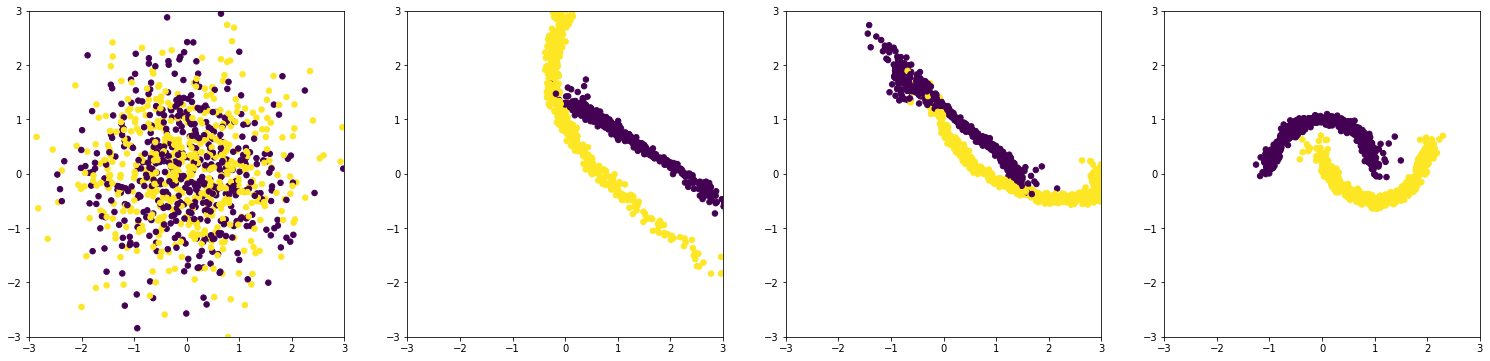
\includegraphics[width=150mm]{figs/two_moons_flow}
%        }
    \end{center}
    \label{fig:moon_flows}
\end{figure}

An additional optional neural network $\tilde{c} = h(c)$ is proposed as a feature extraction model that is trained
end-to-end with the normalizing flow model.
When in use, the coupling block input quantities $c$ are replaced by $\tilde{c}$.
The purpose of the feature extraction network is to efficiently share informative features of the
conditional quantities between all flow layers in favor of each neural network in the flow model independently
extracting informative features.
Inclusion of the network may be important when conditioning on large, complex quantities such as images, however, it
may not be beneficial when conditioning on a small number of simple quantities such as the classification of a hand-drawn
digits or characters.

\section{Generative Adversarial Networks}\label{sec:generative-adversarial-networks}

Generative adversarial networks (GANs)~\cite{gan_goodfellow} are a family of deep generative models characterized by two
distinct models trying to outperform one another.
The goal of a generative model is to construct a probabilistic \textit{generator} $G: \mathbb{R}^k \mapsto \mathbb{R}^n$ such
that samples drawn from $x \sim G$ are ``realistic'' compared to those drawn from a true target distribution $x \sim \pi$.
Determining if a sample is realistic  (i.e. a binary classification to determine if the sample is drawn from $\pi$) is
accomplished with a secondary model referred to as the \textit{discriminator} or critic $D: \mathbb{R}^n \mapsto [0, \; 1]$.
Since $G$ and $D$ are unknown, let $G_\theta$ and $D_\phi$ be functions parameterized by $\theta$ and $\phi$ respectively.

The objective of the discriminator is to correctly classify whether a given observation comes from $G_\theta$ or $\pi$.
Estimating $\phi$ by maximum likelihood yields

\begin{equation}
    \max_{\phi} \underset{x \sim \pi}{\mathbb{E}}\left[ \log D_\phi(x) \right] + \underset{z \sim G_\theta}{\mathbb{E}}\left[ \log \left( 1 - D_\phi(z)\right) \right], \nonumber
\end{equation}
whose expectations can be evaluated via Monte Carlo integration over a set of training observations
$\left\{ x_i \right\}_{i=1}^N \sim \pi$ and a set of synthetic samples $\left\{ z_i \right\}_{i=1}^N \sim G_\theta$.
The objective of the generator is to generate samples that are indistinguishable from samples of $\pi$ as judged by $D_\phi$.
Similarly, estimating $\theta$ by maximimum likelihood yields

\begin{equation}
    \max_{\theta} \underset{z \sim G_\theta}{\mathbb{E}}\left[ \log D_\phi(z) \right].
    \label{eq:adv_loss}
\end{equation}
The expected value in~\eqref{eq:adv_loss} is denoted as the \textit{adversarial loss} function,
$\mathcal{L}_{\text{ADV}}(\theta)$, which can likewise be approximated with a collection of synthetic samples
$\left\{ z_i \right\}_{i=1}^N \sim G_\theta$.

While GANs are widely used for tasks requiring high-dimensional and high-quality samples, they suffer from two key
issues that can severely limit their practicality: unstable training and the phenomenon of \textit{mode-collapse}.

Unstable training arises from the construction of the loss for both the generator and discriminator.
The loss of each model is based on the parameters of the other, thus performing parameter updates during training
results in new loss functions on every update.
The changing objective landscape tends to collapse or diverge during training.
Significant work has gone into improving the stability of GAN training, however, achieving good results is still more
art than science.

The phenomenon of \textit{mode-collapse} is another pervasive problem of GANs, whereby the generator only learns to
generate samples within a small neighborhood of the target distribution resulting in high-quality samples that lack
diversity.
This arises because the generator is only trained to draw samples that have high-likelihood of originating from $\pi$
according to the discriminator, however, it is trivial for the generator to over-fit by generating high-quality samples
only from a small region of the target distribution.
An illustrative example is generating hand-drawn digits, where a \textit{mode-covering} model would be able to generate
realistic images for all digits $0-9$, a \textit{mode-collapsed} model would only be able to generate realistic images
for a subset of digits or only a single digit.

\section{Flow-GAN}\label{sec:flow-gan}

The Flow-GAN~\cite{flow_gan} model proposes using a normalizing flow for the generator function to overcome the two
key issues presented with GANs by constructing a hybrid loss function for the generator combining both the
\textit{maximum-likelihood loss} and \textit{adversarial loss} functions,

\begin{equation*}
    \min_{\theta} \mathcal{L}_{\text{MLE}}(\theta) - \lambda_{\text{ADV}} \mathcal{L}_{\text{ADV}}(\theta),
    \label{eq:flowgan_loss}
\end{equation*}
where $\lambda_{\text{ADV}} \geq 0$ is a hyperparameter used to blend the losses.
Setting $\lambda_{\text{ADV}} = 0$ is equivalent to training a vanilla normalizing flows model ignoring the discriminator,
while setting $\lambda_{\text{ADV}}$ to a large number is equivalent to training a vanilla GAN\@.

Inclusion of $\mathcal{L}_{\text{MLE}}$ alleviates both unstable training and mode-collapse issues.
First, the optimization landscape of $\mathcal{L}_{\text{MLE}}$ is constant with respect to the parameters $\phi$ and
$\theta$, thus convergence of the generator with respect to how well it captures the sample target distribution from the
training observations can be monitored throughout training.
Second, maximizing the likelihood of observing all training examples means mode-collapse is unlikely as any collapse
during training would be heavily penalized with extremely low likelihood evaluations.
